% Copyright (C) 2007 by Ignacio Llopis <lloptor@gmail.com>
% -------------------------------------------------------
% 
% This file contains an example of what paperTeX class can do.
% Compile it using PDFLaTeX in order to get the best results.
% This file requires the img/ folder.
% There are many comments that the user can uncomment in order to see 
% how easy is to change the output style.
%
%
% This file may be distributed and/or modified under the
% conditions of the LaTeX Project Public License, either version 1.2
% of this license or (at your option) any later version.
% The latest version of this license is in:
%
%    http://www.latex-project.org/lppl.txt
%
% and version 1.2 or later is part of all distributions of LaTeX 
% version 1999/12/01 or later.

\documentclass[10pt,final]{papertex}

\usepackage[latin1]{inputenc}
\usepackage[english]{babel}
%\usepackage[T1]{fontenc}
\usepackage{ulem}
\usepackage{color}
\usepackage{times}
\usepackage{mathptmx}
\usepackage[11pt]{moresize}
\usepackage{graphicx}
\usepackage{fancyhdr}
\usepackage{multicol}
\usepackage[linewidth=1pt]{mdframed}
\definecolor{color}{cmyk}{1, 0,0, 0.8}
\foot{All the lastest information can be found on:}{\href{http://aims.robots.ox.ac.uk}{aims.robots.ox.ac.uk}}{}

%\renewcommand{\indexEntryFormat}{\large\rmfamily}
%\renewcommand{\indexEntryPageTxt}{page}
%\renewcommand{\timestampSeparator}{$\Rightarrow$}
%\renewcommand{\innerTextFinalMark}{$\spadesuit$}

\newcommand\textline[4][t]{%
	\par\smallskip\noindent\parbox[#1]{.333\textwidth}{\raggedright\texttt{+}#2}%
}
\renewcommand{\logo}{\mylogo{\noindent{\fontsize{10mm}{14mm} \usefont{T1}{pag}{m}{n} \textcolor{black}{AIMS CDT Newsletter}}\\[3pt]}}
\renewcommand{\minilogo}{}
\renewcommand{\editionFormat}{\LARGE}
\renewcommand{\indexEntryFormat}{\normalsize\rmfamily}

\author{}
\title{AIMS Quarterly update}
\edition{Jan - Jul Edition}

%\setlength{\columnsep}{2cm}


%new "ragged text" feature
\minraggedcols=3

\begin{document}

%\maketitle

\begin{frontpage}
\begin{figure}
    \mbox{
\includegraphics{img/aims1}}   
\hspace{25px}
\mbox{
\includegraphics{img/aims2}}
\hspace{25px}
\mbox{
\includegraphics{img/aims3}}
\end{figure}
\vspace{1cm}
\noindent\mbox{%
	\parbox{\textwidth}{%
	\huge{A} \large{warm welcome to all our industrial partners and to our new partners: $\textit{\textbf{ABB}}$, $\textit{\textbf{Samsung}}$ and $\textit{\textbf{Toshiba}}$. We thank you all for your continued support and wish to showcase to you, the amazing work that is currently being undertaken in the EPSRC \textbf{C}entre for \textbf{D}octoral \textbf{T}raining in \textbf{A}utonomous \textbf{I}ntelligent \textbf{M}achines and \textbf{S}ystems. With the introduction of our new half-yearly student led newsletter, we hope to keep you informed and updated with research that is currently being undertaken and its potential applications for industry.  }
	}%
}	
\noindent\mbox{%
	\raggedright
	\parbox{\textwidth}{%
		\vspace{0.5cm}
		\textbf{T}\large{he AIMS program combines research from  a plateau of domains. From autonomous vehicles, to visual recognition and object detection, sensor networks, smart buildings, 3D reconstruction, multi-agent systems, reinforcement learning, Bayesian inference, probabilistic programming and much, much more.   }
	}%
}
\\
\section*{Robotics Week}
\noindent
\begin{multicols}{2}
	\noindent\textbf{D}\large{uring robotics week the new first year cohort split into three teams and worked together, with the aim to create and build a system that would allow a husky robot to navigate completely autonomously through three obstacle based challenges.
	Teams had to put the theory that they had learnt to the test and apply that knowledge to a real world system.\\
	
	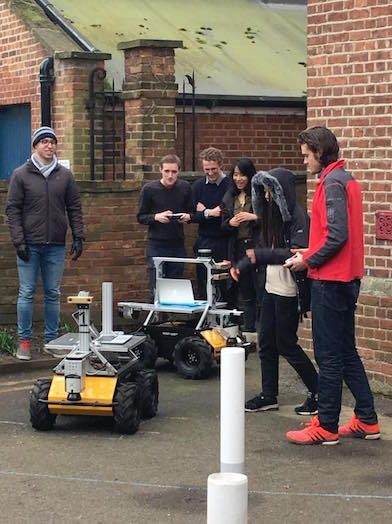
\includegraphics[width=6cm,height=6cm,keepaspectratio]{img/robots}
%	\caption{\\\small{Two teams preparing their huskies for the 2nd challenge}}
    
    \noindent The first obstacle course was target detection, can the husky spot the goal and drive to it autonomously. The second was to navigate round a series of obstructions, correctly identify the target and then drive back. The third was similar to the second, but with more obstacles.\\
    \noindent The competition was fierce and the final scores were close, but team three were the victors.\\
     
	\noindent 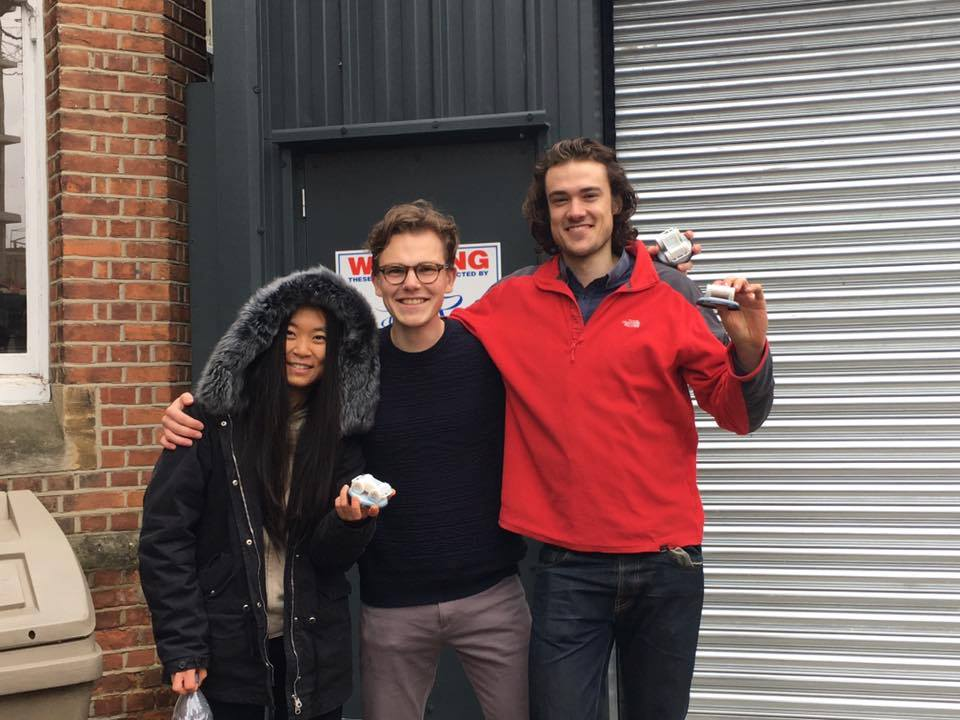
\includegraphics[width=6cm,height=6cm,keepaspectratio]{img/winning}
    \caption{\\\small{Team 3. From left to right: Xu Ji, Adam Goli\'nski, Oliver Bent}} 
	}
\end{multicols}
\begin{mdframed}[leftmargin=7pt,rightmargin=7pt]
	\textbf{EDITORS}\\
	Bradley Gram-Hansen \textbf{||} AIMS student (1st year) \textbf{||} \href{mailto:bradley@robots.ox.ac.uk}{\texttt{bradley@robots.ox.ac.uk}}\\
	Wendy Adams \hspace{1cm}       \textbf{||} AIMS administrator \hspace{0.5cm} \textbf{||} \href{mailto:wendy.adams@eng.ox.ac.uk}{\texttt{wendy.adams@eng.ox.ac.uk}}\\
	
\end{mdframed}


%\begin{indexblock}{MAIN INDEX}
%\indexitem{$\textbf{Internships}$}{1}
%
%\indexitem{$\textbf{Papers submitted 2017}$}{1}
%
%\indexitem{$\textbf{Future work}$}{2}
%
%
%\end{indexblock}

%\begin{weatherblock}{WEATHER FORECAST}
%\weatheritem{img/weather/rain.jpg}{TODAY}{13}{9}{}
%\weatheritem{img/weather/sun.jpg}{TOMORROW}{15}{11}{}
%\weatheritem{img/weather/clouds.jpg}{FRIDAY}{12}{6}{}
%\end{weatherblock}


\end{frontpage}

\newsection{}

\begin{news}{1}
	{Internships}
	{}
	{}
	{2}
%\authorandplace{Name Surname}{Place}

%\image{img/aims2}{News image caption.}
\columntitle{lines}{AIMS students are embarking
on a wide range of internships this year}

\textbf{S}tefan Safetscu (3rd year) will be an intern for \textbf{Google} in California. Adam Cobb (2nd year) and Tim Seabrook (2nd year) will be both interning for \textbf{NASA}s Frontier Development Lab (FDL) in Mountain view, California. 
Oliver Bent (1st year) will be traveling to Kenya to work with \textbf{IBM Africa} on Mosquito detection. 
\end{news}

\newssep

\begin{news}{1}
	{Papers Submitted to 2017 Conferences}
	{}
	{}
	{1}
\columntitle{lines}{AIMS students have had a successful year so far}
\noindent in both submitting and having papers accepted for this years big machine learning, computer vision and programming conferences, such as: NIPS, ICML, ICLR, ECML, POPL and ICCV.\\

Adam Cobb (2nd year student), who submitted the following to NIPS:\hspace{0.1mm} \textbf{Learning from  lions: inferring the utility of agents from their trajectories}.\\
The paper used GPS data from lions in order to make inferences about their preferences over waterholes, fences and other significant features.

\noindent Greg Farquhar (2nd year) and Triantafyllos Afouras (1st year), jointly submitted to NIPS this year, with a paper on multi-agent reinforcement learning:\hspace{0.1mm}\textbf{ Counterfactual Multi-Agent Policy Gradients}.\\
In the paper they train neural networks to play the computer game StarCraft, treating each unit as an independent agent with limited, local information. The algorithms are relevant for any context in which you can have centralised training, but the agents need to execute decentralised policies. The work could be used to help optimise the coordination of drones or autonomous vehicles.\\
Nikitas Rontsis (2nd year) also submitted to NIPS this year, with a paper: \textbf{Distributionally Robust Optimization Techniques in Batch Bayesian Optimization}.\\
 The paper  uses ideas from Convex Optimisation and Control theory, and applies them to Machine Learning techniques, with an emphasis to Gaussian Processes. Applications include Bayesian Optimisation and safety critical dynamical systems.\\
 Robert Cornish (2nd year) submitted two papers to NIPS \textbf{Online Learning Rate Adaptation with Hypergradient Descent } and \textbf{On the Opportunities and Pitfalls of Nesting Monte Carlo Estimators}.\\
 Finally, James Thewlis (3rd year) submitted to NIPS with \textbf{ Unsupervised object learning from dense equivariant image labelling}\\
 
 To ECML Ivan Kiskin (2nd year) submitted \textbf{Mosquito Detection with Neural Networks The Buzz of Deep Learning}\\
 
 
L\'eonard Berrada (2nd year) had his publication to ICLR 2017 \textbf{accepted}, which created a more efficient optimisation algorithm for  Piecewise-Linear Convolutional Neural Networks (PL-CNNs), which enables better classification of objects within images. The paper is called \textbf{Trusting SVM for Piecewise Linear CNNs}\\
%\expandedtitle{doublebox}{This is an expanded ``doublebox'' }

To ICCV James Thewlis submitted a paper for learning representations of objects called \textbf{Unsupervised learning of object landmarks by factorized spatial embeddings}\\
Where with as little as 5 marked points and 20 training samples, it was possible to learn what a face is, or what characterises a shoe or a fox.\\

Greg Farquhar and Triantafyllos Afouras have had thier paper on multi-agent reinforcement learning \textbf{accepted} for ICML 2017. Their paper \textbf{Stabilising Experience Replay for Deep Multi-Agent Reinforcement Learning} has potential applications for urban traffic control and network packet routing, among others. \\

Robert Cornish had his paper \textbf{Efficient exact inference in discrete Anglican programs.} for the PPS workshop at POPL 2017 \textbf{accepted}  \\

Siddarth Ghoshal has had his paper \textbf{Reading the Tea Leaves: A Neural Network Perspective on Technical Trading} published in KDD (Knowledge Discovery and Data, 2017) \textbf{accepted}.
\end{news}

\newssep

\newsection{SECTION B}


\begin{news}{2}
	{Current Projects}
	{The current first year students have competed their first mini-projects which took place over the Easter Vacation.  Below are the subjects they have been working on. }
	{SECTION B}
	{2}

%\authorandplace{Name Surname}{Place}

%\image{img/ireland}{Image caption.}

\noindent 
\begin{itemize}
\item Counterfactual multi-agent policy gradients\\
\item Improving exploration in deep reinforcement learning\\
\item Forecasting financial time series with CNNs\\
\item Neural networks for 2D to 3D human pose estimation\\
\item Multi-layer stacked Gaussian Processes\\
\item Seeing is believing: Contrastive hebbian clustering for unsupervised one-shot gameplay learning in a recurrent neural network\\
\item Inference of spatial distribution from multi-sensor measurements along trajectories with inaccurate location information\\
\item Closed-loop quantitative verification of rate-adaptive pacemakers\\
\item Learning from limited demonstrations in high dimensional feature spaces\\
\item Meta-probabilistic numerics\\
\end{itemize}

%Integer interdum ultricies justo. Nam at sem et felis fringilla faucibus. Suspendisse varius, mauris sit amet pretium fermentum, arcu massa interdum metus, a varius justo ante sed velit. Class aptent taciti .
%
%Sed sit amet lectus. Suspendisse scelerisque. Donec nisl quam, mattis eu, lobortis eu, varius eget, 
%
%Ut convallis consectetuer odio. Fusce posuere eleifend arcu. Nullam libero turpis, porttitor pellentesque, dictum vulputate, varius ut, turpis. Sed facilisis, nisi nec commodo commodo, enim risus 
%
%\expandedtitle{lines}{Another expanded title. Suspendisse scelerisque. Donec nisl quam, mattis eu, lobortis eu, varius eget, urna.}

%Proin sollicitudin volutpat quam. Duis pulvinar nulla id lorem. Curabitur ac nulla eget dui porta laoreet. Integer turpis mauris, dignissim quis, faucibus sit amet, placerat quis, odio. Mauris blandit, 

%Donec ultrices sem non ante. Curabitur non ante vitae mauris eleifend convallis. Integer lectus lorem, 
\end{news}

\newssep

%\begin{editorial}{1}{This is an example of ``editorial'' type of news.}{Name Surname}{4}
%Proin sollicitudin volutpat quam. Duis pulvinar nulla id lorem. Curabitur ac nulla eget dui porta 
%
%Donec ultrices sem non ante. Curabitur non ante vitae mauris eleifend convallis. Integer lectus lorem, scelerisque et, dictum sollicitudin, aliquam a, eros. Ut ultrices metus eu augue. Cras sit amet odio sit amet dolor sagittis venenatis. Vestibulum ante ipsum primis in faucibus orci luctus et ultrices posuere cubilia Curae; Aliquam erat volutpat. Sed justo velit, accumsan sed, vulputate nec, nonummy sed, tellus. Phasellus sit amet odio sed erat placerat posuere. Sed a magna. Cras dolor turpis, consequat sollicitudin, viverra eget, convallis eu, nibh.
%
%Ut convallis consectetuer odio. Fusce posuere eleifend arcu. Nullam libero turpis, porttitor pellentesque, dictum vulputate, varius ut, turpis. Sed facilisis, nisi nec commodo commodo, enim risus ultrices leo, non tristique nibh dolor a dolor. Etiam placerat justo non felis. Suspendisse pulvinar nisl a magna. Vivamus dapibus nulla quis felis. Nulla luctus dignissim nisi. Curabitur sit amet nibh. Etiam pulvinar.
%\end{editorial}

\newssep

%\begin{shortnews}{4}{SHORT NEWS ENVIRONMENT}{The shortnews environment inside \TeX{}}{5}
%\shortnewsitem{This is a short title}{This is a short text. Lorem ipsum dolor sit amet, consectetuer adipiscing elit. In vitae augue. Morbi fermentum, felis accumsan rhoncus malesuada, metus eros adipiscing dui, vel eleifend nibh velit ut felis. Pellentesque elementum massa at nisi dapibus mollis. Etiam cursus. Mauris gravida nibh ut sapien. Vestibulum pretium, felis et.}
%\shortnewsitem{Another short title}{This is a short text. Lorem ipsum dolor sit amet, consectetuer adipiscing elit. In vitae augue. Morbi fermentum, felis accumsan rhoncus malesuada, metus eros adipiscing dui, vel eleifend nibh velit ut felis. Pellentesque elementum massa at nisi dapibus mollis. Etiam cursus. Mauris gravida nibh ut sapien. Vestibulum pretium, felis et.}
%\shortnewsitem{This is a short title}{This is a short text. Lorem ipsum dolor sit amet, consectetuer adipiscing elit. In vitae augue. Morbi fermentum, felis accumsan rhoncus malesuada, metus eros adipiscing dui, vel eleifend nibh velit ut felis. Pellentesque elementum massa at nisi dapibus mollis. Etiam cursus. Mauris gravida nibh ut sapien. Vestibulum pretium, felis et.}
%\shortnewsitem{Another short title}{This is a short text. Lorem ipsum dolor sit amet, consectetuer adipiscing elit. In vitae augue. Morbi fermentum, felis accumsan rhoncus malesuada, metus eros adipiscing dui, vel eleifend nibh velit ut felis. Pellentesque elementum massa at nisi dapibus mollis. Etiam cursus. Mauris gravida nibh ut sapien. Vestibulum pretium, felis et.}
%\shortnewsitem{This is a short title}{This is a short text. Lorem ipsum dolor sit amet, consectetuer adipiscing elit. In vitae augue. Morbi fermentum, felis accumsan rhoncus malesuada, metus eros adipiscing dui, vel eleifend nibh velit ut felis. Pellentesque elementum massa at nisi dapibus mollis. Etiam cursus. Mauris gravida nibh ut sapien. Vestibulum pretium, felis et.}
%\shortnewsitem{Another short title}{This is a short text. Lorem ipsum dolor sit amet, consectetuer adipiscing elit. In vitae augue. Morbi fermentum, felis accumsan rhoncus malesuada, metus eros adipiscing dui, vel eleifend nibh velit ut felis. Pellentesque elementum massa at nisi dapibus mollis. Etiam cursus. Mauris gravida nibh ut sapien. Vestibulum pretium, felis et.}
%\end{shortnews}

%\newssep
%\newssep
\end{document}